\section{Evaluation Setup and Metric Definitions}
\label{app:evaluation_setup}
This appendix provides the full evaluation protocol summarized in~\cref{subsec:setup}: the prompt construction pipeline for direct, indirect, neighbor, and control evaluation; formal definitions of the seven metrics used in~\cref{sec:experiment}; and the classification vocabulary shared across all experiments.

\subsection{Prompt Construction and Scoring Pipeline}
\label{app:eval_pipeline}
Our automated evaluation protocol is designed to measure two coupled consequences of concept entanglement: \emph{indirect recovery}, where an erased concept remains recoverable through correlated contextual cues, and \emph{collateral forgetting}, where suppressing a target concept degrades performance on nearby concepts that should remain intact. To distinguish these effects, we separately construct (i) direct prompts that explicitly name $c$, (ii) indirect prompts constructed from correlated context without naming $c$, (iii) neighbor prompts that explicitly name each concept in the neighborhood $\mathcal{N}(c)$, and (iv) control prompts that name each concept in the control set $\mathcal{C}(c)$.

\paragraph{Correlated context extraction.}
For each target concept $c$, we collect a target-matched caption subset from LAION~\citep{schuhmann2022laion} aligned with diffusion-model pretraining. Specifically, we identify captions that explicitly contain $c$ or its lexical variants, and extract co-occurring content words and short phrases from this subset. We remove stopwords, punctuation, low-information function words, and lexical forms that directly mention the target concept. The remaining candidates are ranked using corpus-level association statistics and filtered to obtain a final set of correlated context words that captures the contextual footprint of $c$ in the training distribution. For example, when $c=\texttt{horse}$, the resulting set includes terms such as \texttt{jockey}, \texttt{stable}, \texttt{saddle}, \texttt{racetrack}, and \texttt{polo}, for $c = \texttt{castle}$, it includes \texttt{moat}, \texttt{turret}, \texttt{medieval}, \texttt{knight}, and \texttt{drawbridge}.

To visualize how these correlated prompts organize in text-embedding space, we pool prompts that explicitly mention the target concept and prompts that omit the target token but retain correlated context, then project their CLIP text embeddings to two dimensions with PCA. \Cref{fig:bow_context_span} shows that context-rich prompts occupy a nearby region rather than a disjoint cluster, supporting our bag-of-words motivation that concept evidence is distributed across correlated tokens rather than isolated in a single concept word.

\begin{figure}[t]
\centering
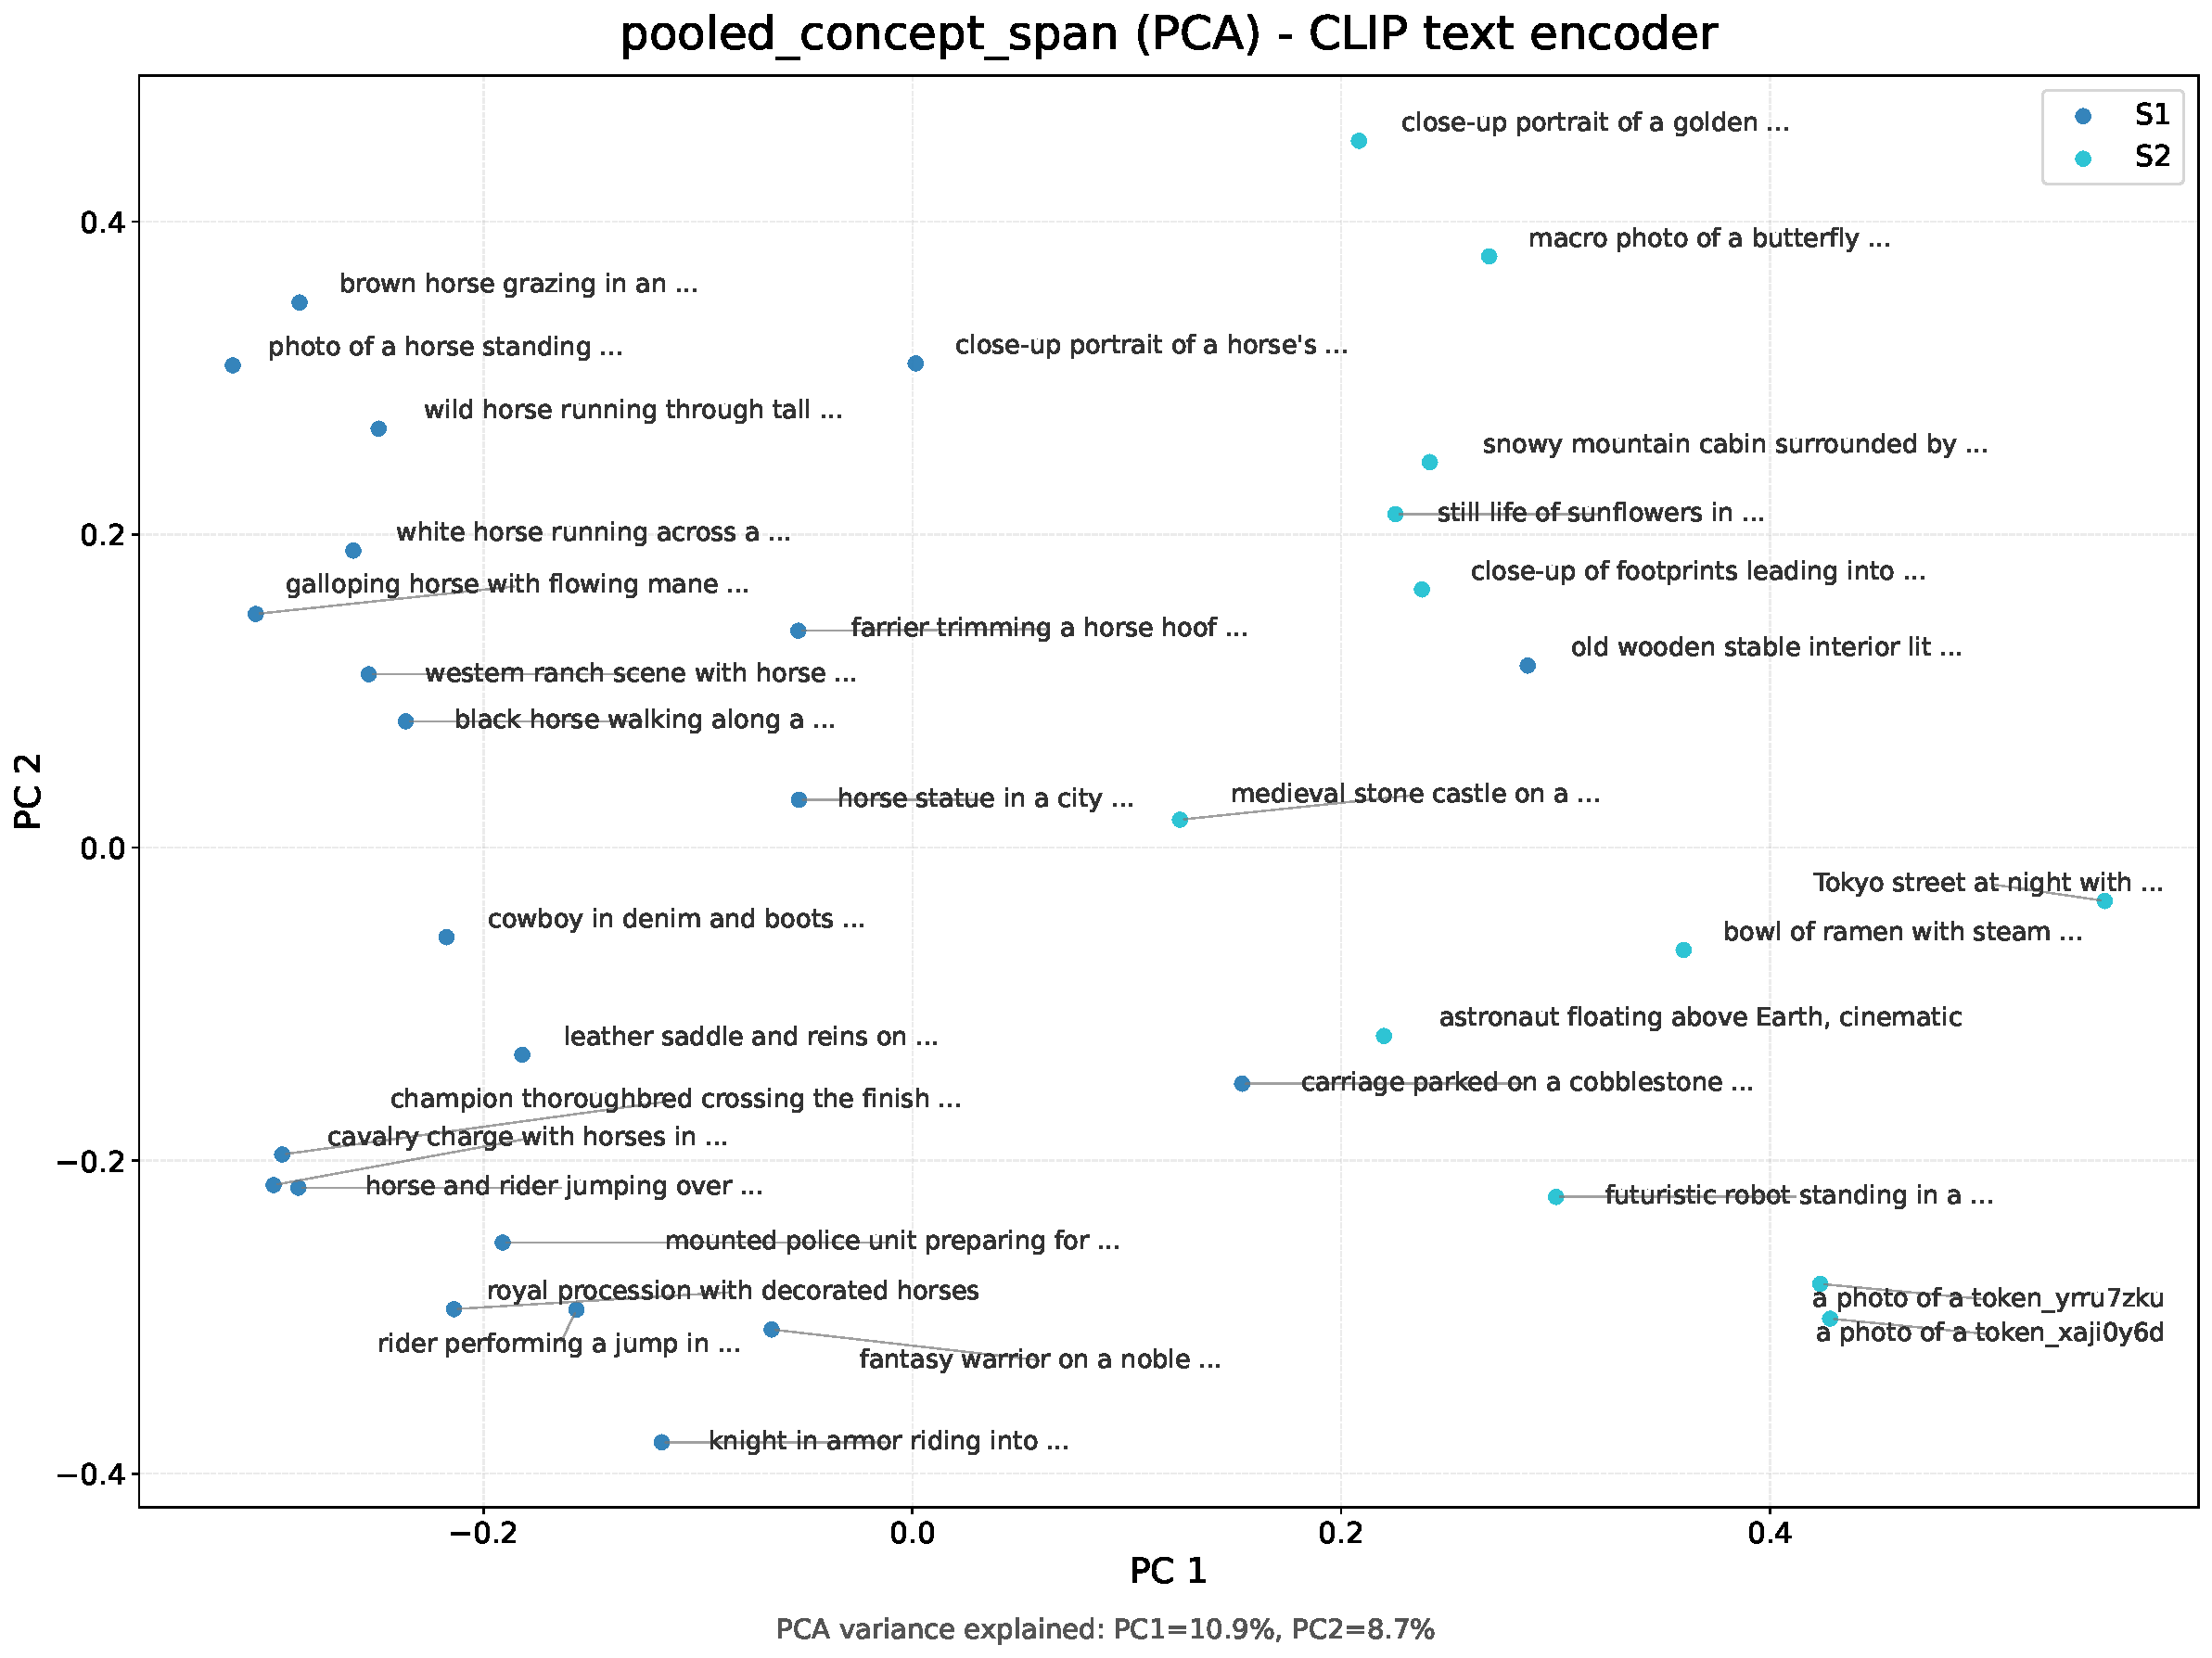
\includegraphics[width=\linewidth]{img/bag_of_words_span.pdf}
\caption{
\textbf{Context-only prompts remain close to target prompts in CLIP text-embedding space.}
PCA projection of pooled prompts used for the \texttt{horse} case study. One group explicitly contains the concept token, while the other omits it but retains correlated context words (e.g., \texttt{jockey}, \texttt{saddle}, \texttt{racetrack}). The proximity between these groups illustrates why token-level erasure can remain vulnerable to indirect contextual prompts.
}
\label{fig:bow_context_span}
\end{figure}


\paragraph{Indirect recovery prompts.}
We use the correlated context set for $c$ to construct a set of indirect prompts $\mathcal{P}_{\mathrm{ind}}(c)$. These prompts are generated under an explicit lexical exclusion constraint: they must not contain the target token or excluded lexical variants of $c$. Intuitively, $\mathcal{P}_{\mathrm{ind}}(c)$ probes whether the erased concept can still be elicited through contextual associations alone, without direct lexical mention. To improve prompt diversity while preserving control, we generate multiple prompts from different subsets of the correlated context words and retain only prompts that satisfy the exclusion rule.

\paragraph{Semantic neighbors and control concepts.}
The semantic neighborhood $\mathcal{N}(c)$ is determined by the universal-pool $\delta$-threshold procedure given in~\cref{def:semantic_neighborhood}: $\mathcal{N}(c)$ collects all candidates in the shared pool $\mathcal{C}_{\mathrm{pool}}$ whose centroid cosine distance to $c$ falls below the global 25th-percentile threshold $\delta$. This produces concept-specific neighborhoods of five to seven discovered neighbors per target (\cref{tab:kappa_per_target}).
The control set $\mathcal{C}(c) = \{\texttt{airplane}, \texttt{bicycle}, \texttt{cactus}, \texttt{jellyfish}, \texttt{lighthouse}, \texttt{melon}, \texttt{police car}, \texttt{teapot}, \texttt{violin}, \texttt{volcano}\}$ is identical across all five targets and consists of concepts whose centroids lie well above $\delta$ for every target, verified to contribute zero to $\hat\kappa$ across all five targets. For each neighbor $c' \in \mathcal{N}(c)$ and control $\tilde c \in \mathcal{C}(c)$, we generate prompts that explicitly mention the concept while excluding lexical forms of the target $c$. Per-target prompt files are released in the supplementary material.

\paragraph{Classifier-based scoring.}
All images are classified using a CLIP-based classifier over a fixed vocabulary of 65 concept labels (\cref{app:vocab}). For each image, the classifier returns the top-1 label among the vocabulary. All metrics defined below are computed from these top-1 assignments. In several random instances, we also perform a manual evaluation to ensure consistency of the results.

% For each prompt set, we generate images from the base model $\mathcal{D}_\theta$ and each unlearned model $\mathcal{D}_{\hat{\theta}}$, and evaluate the outputs using a pretrained concept classifier. For indirect prompts, we measure the fraction of generated images classified as the erased concept $c$, yielding an estimate of indirect recovery. For neighbor prompts, we measure classifier accuracy on the intended neighbor concept $c'$, which captures neighbor preservation after unlearning. For control prompts, we analogously measure accuracy on the intended non-neighbor control concept. Together, these scores allow us to distinguish target-specific collateral damage on semantic neighbors from broader degradation on unrelated concepts.

\subsection{Evaluation Metrics}
\label{app:metric_defs}
Each metric is defined with respect to a base model 
$\mathcal{D}_\theta$ and an unlearned model 
$\mathcal{D}_{\hat\theta}$. We write $\mathrm{Acc}(\mathcal{D}, c, \mathcal{P})$ for the fraction of images generated by model $\mathcal{D}$ from prompts in set $\mathcal{P}$ that are classified as concept $c$ by the CLIP evaluator.

\paragraph{Erasure metrics (measuring $\varepsilon$).}
These metrics measure how effectively the target concept $c$ is suppressed in the unlearned model.
\begin{itemize}
    \item \emph{Unlearning Accuracy (UA)}: The fraction of images generated from direct prompts $\mathcal{P}_{\mathrm{dir}}(c)$ by $\mathcal{D}_{\hat\theta}$ that 
    are \emph{not} classified as $c$. 
    \begin{equation}
    \label{eq:ua}
    \mathrm{UA}(c) = 1 - \mathrm{Acc}(\mathcal{D}_{\hat\theta}, c, \mathcal{P}_{\mathrm{dir}}(c)).
    \end{equation}
    Higher UA indicates more complete erasure under explicit lexical prompts.
    \item \emph{Indirect Recovery Rate (IRR)}: The fraction of images generated from indirect recovery prompts $\mathcal{P}_{\mathrm{ind}}(c)$ by 
    $\mathcal{D}_{\hat\theta}$ that \emph{are} classified as $c$: 
    \begin{equation}
    \label{eq:irr}
    \mathrm{IRR}(c) = \mathrm{Acc}(\mathcal{D}_{\hat\theta}, c, \mathcal{P}_{\mathrm{ind}}(c)).
    \end{equation}
    Higher IRR indicates greater vulnerability to concept recovery through correlated contextual cues. In contrast to UA, IRR measures the $\varepsilon$-robust erasure property formalized in~\cref{def:robust}.
\end{itemize}

\paragraph{Retention metrics (measuring $\gamma$).}
We measure retention at three levels of granularity:
\begin{itemize}
    \item \emph{In-domain Retain Accuracy (IRA)}: The fraction of images generated from indirect prompts by $\mathcal{D}_{\hat\theta}$ that are classified as a non-target, non-neighbor, non-control concept in the vocabulary. This captures the tendency of an unlearned model to substitute unrelated concepts when indirectly prompted for the erased target.
    %\ali{are we using this metric only for the UnlearnCanvas dataset? if not, this part is confusing and not needed.
    \item \emph{Neighbor Preservation (NP)}: This is our primary trade-off metric. The overlap with remaining concepts is often dominated by the overlap with a few concepts which are mostly semantically similar with the target concept. Therefore, as a proxy metric for utility preservation, we evaluate utility preservation in the semantic neighborhood $\mathcal{N}(c)$ of the target concept (\cref{def:semantic_neighborhood}) and define
    \begin{equation}
    \label{eq:neighbor_pres}
    \mathrm{NP}(c) = \frac{1}{|\mathcal{N}(c)|} \sum_{c' \in \mathcal{N}(c)} \frac{\mathrm{Acc}(\mathcal{D}_{\hat\theta}, c', \mathcal{P}_{\mathrm{dir}}(c'))}
    {\mathrm{Acc}(\mathcal{D}_\theta, c', \mathcal{P}_{\mathrm{dir}}(c'))}.
    \end{equation}
    An NP score of $1.0$ indicates perfect preservation of neighbors after unlearning; lower values indicate proportional collateral damage. The ratio form normalizes out the base-model recognition accuracy, which differs across concepts (and which is generally below 1.0 under a 65-class vocabulary).
    % where $\mathrm{Acc}(\mathcal{D}, c')$ denotes classifier accuracy on prompts for concept $c'$ under model $M$. An NP score of 1.0 indicates perfect preservation of nearby concepts, while lower values indicate stronger collateral damage. Unlike IRA, which averages over all non-target concepts, NP focuses specifically on semantically nearby concepts that are most likely to overlap with the erased target. \textbf{Relation to $\gamma$.} NP is an operational, classifier-based proxy for the activation-level neighbor preservation error $\gamma$ in Definition~\ref{def:neighbor}. By Assumption~\ref{asm:lip}, a small activation displacement $\|\Phi_{\hat\theta}(p) - \Phi_\theta(p)\|_2$ induces a small change in concept generation probability and hence a small drop in classifier accuracy; conversely, a method that preserves $\mathrm{NP} \approx 1$ must have kept activations close in $\mathcal{H}$. NP and $1-\gamma$ therefore track the same underlying quantity up to the Lipschitz constant $L$ and classifier noise, which is what makes it the right axis against which to plot Theorem~\ref{thm:tradeoff}'s predicted Pareto frontier.
    \item \emph{Control preservation (CP)}: To distinguish neighbor-specific collateral damage from broader degradation, we additionally evaluate performance on a non-neighbor control set $\mathcal{C}(c)$. We define
    \begin{equation}
    \label{eq:cp}
    \mathrm{CP}(c) = \frac{1}{|\mathcal{C}(c)|} \sum_{\tilde c \in \mathcal{C}(c)} 
    \frac{\mathrm{Acc}(\mathcal{D}_{\hat\theta}, \tilde c, \mathcal{P}_{\mathrm{dir}}(\tilde c))}
     {\mathrm{Acc}(\mathcal{D}_\theta, \tilde c, \mathcal{P}_{\mathrm{dir}}(\tilde c))}.
    \end{equation}
    Comparing NP and CP isolates neighbor-specific collateral damage from broader degradation: a method with $\mathrm{NP} \ll \mathrm{CP}$ is damaging concepts selectively in the target's neighborhood, consistent with the propagation mechanism in~\cref{thm:tradeoff}. A method with $\mathrm{NP} \approx \mathrm{CP} \ll 1$ is causing uniform degradation across the concept space.
    % where $\tilde{c}$ denotes a control concept that is semantically distant from $c$. Comparing NP and CP allows us to determine whether a method disproportionately harms nearby concepts, rather than causing uniform degradation across the concept space.
\end{itemize}


% \paragraph{Image quality.}
% We report Fr'{e}chet Inception Distance (FID)~\citep{heusel2017gans} to verify that the observed tradeoffs are not merely artifacts of overall image-quality degradation.


\paragraph{DamageGap.} A summary statistic we introduce to quantify neighbor-selective damage: $\mathrm{DamageGap}(c) = \mathrm{CP}(c) - \mathrm{NP}(c)$. A positive DamageGap indicates that neighbors are damaged more than controls, consistent with the trade-off predicted by~\cref{thm:tradeoff}. A DamageGap near zero indicates uniform degradation (or uniform preservation) across both sets.

\subsection{Classification Vocabulary}
\label{app:vocab}
All CLIP-based classification uses the following 65-concept vocabulary, which is identical to the universal candidate pool $\mathcal{C}_{\mathrm{pool}}$ used for $\hat\kappa$ estimation (\cref{app:kappa_estimation}).
The same vocabulary is used for every metric and every target, ensuring cross-target comparability.

\begin{table}[h]
\centering
\small
\begin{tabular}{p{3.2cm} p{10cm}}
\toprule
Category & Concepts \\
\midrule
Targets & \texttt{horse}, \texttt{cat}, \texttt{dog}, \texttt{bear}, \texttt{castle} \\
Equine  & \texttt{pony}, \texttt{donkey}, \texttt{zebra}, \texttt{mustang}, \texttt{mare}, \texttt{foal}, \texttt{stallion}, \texttt{mule}, \texttt{bison}, \texttt{camel} \\
Feline  & \texttt{kitten}, \texttt{tiger}, \texttt{lion}, \texttt{leopard}, \texttt{panther}, \texttt{cheetah}, \texttt{lynx}, \texttt{jaguar}, \texttt{cougar}, \texttt{bobcat} \\
Canid  & \texttt{puppy}, \texttt{fox}, \texttt{coyote}, \texttt{jackal}, \texttt{dingo}, \texttt{hyena}, \texttt{husky}, \texttt{labrador}, \texttt{beagle}, \texttt{retriever} \\
Ursine & \texttt{grizzly}, \texttt{polar bear}, \texttt{panda}, \texttt{cub}, \texttt{koala}, \texttt{black bear}, \texttt{brown bear}, \texttt{teddy bear}, \texttt{sloth bear}, \texttt{sun bear} \\
Architectural  & \texttt{fortress}, \texttt{tower}, \texttt{cathedral}, \texttt{palace}, \texttt{keep}, \texttt{citadel}, \texttt{watchtower}, \texttt{stronghold}, \texttt{fortified wall}, \texttt{manor} \\
Controls  & \texttt{airplane}, \texttt{bicycle}, \texttt{cactus}, \texttt{jellyfish}, \texttt{lighthouse}, \texttt{melon}, \texttt{police car}, \texttt{teapot}, \texttt{violin}, \texttt{volcano} \\
\bottomrule
\end{tabular}
\caption{The $65$-concept classification vocabulary used for all CLIP-based metric evaluations in~\cref{sec:experiment}. The vocabulary is the union of the five targets, their respective fine-grained subtype candidates spanning four animal category and one architectural category, and ten out-of-domain controls. See~\cref{tab:kappa_per_target} for the per-target subset $\mathcal{N}(c) \subseteq \mathcal{C}_{\mathrm{pool}}$ that survives the $\delta$-filter and forms the averaging set for NP.}
\label{tab:vocab}
\end{table}
